\documentclass[12pt,a4paper]{article}
\usepackage[legalpaper, portrait, margin=3cm]{geometry}
\usepackage{fancyhdr}
\usepackage{amsmath}
\usepackage{amssymb}
\usepackage{graphicx}
\usepackage{blindtext}
\usepackage{hyperref}
\usepackage{indentfirst}
\usepackage{biblatex}

\graphicspath{ {./} }
\hypersetup{
  colorlinks=true,
  linkcolor=blue,
  filecolor=magenta,
  urlcolor=blue,
  citecolor=blue,
  pdftitle={Relatório ASA Projeto 2 2022/2023},
  pdfpagemode=FullScreen,
}
\addbibresource{./bibliography.bib}

\pagestyle{fancy}
\fancyhf{}
\rhead{Grupo \textbf{al013}}
\lhead{Relatório ASA Projeto 2 2022/2023 LEIC-A}
\cfoot{Gonçalo Sampaio Bárias (103124)}

\renewcommand{\footrulewidth}{0.2pt}

\renewcommand{\labelitemii}{$\circ$}
\renewcommand{\labelitemiii}{$\diamond$}

\begin{document}
  \section{Descrição do Problema e da Solução}

  O problema proposto foi o de ajudar um governo num país imaginário, Caracolândia, a encontrar o número máximo de trocas comerciais entre regiões vizinhas passíveis de serem transportadas para uma rede ferroviária, minimizando os custos de financiamento dos troços ferroviários.

  Para resolver o \textbf{problema} recorreu-se a uma implementação modificada do algoritmo de Kruskal para minimizar a quantidade de arestas num grafo, maximizando o seu peso.
  O problema é modelado por um \textbf{grafo de pesos não direcionado} e por isso podemos aplicar o algoritmo mencionado.
  Um \textbf{vértice} no grafo representa uma \textbf{região} no país imaginário.
  Uma \textbf{aresta} representa uma \textbf{conexão entre duas regiões}, entre as quais existem \textbf{trocas comerciais}, que representam o \textbf{peso} dessa aresta.

  Assim, na modelação da solução, a informação das arestas recebida como input é representada por uma \textit{struct} que guarda os identificadores dos dois vértices e o peso dessa aresta.
  O algoritmo começa por ordenar as arestas do grafo pelo seu peso em ordem decrescente, pois assim permite ao algoritmo de Kruskal escolher sempre, das arestas que faltam, a que tem o maior número de trocas comerciais.
  Em seguida, percorre o vetor ordenado e adiciona vértices a uma estrutura de dados designada por \textbf{conjunto disjunto}.
  O algoritmo utiliza a estrutura de dados para garantir que apenas liga à árvore as arestas que não criam ciclos.
  Faz isto, utilizando a operação \texttt{findSet} para verificar se os dois vértices de uma aresta já se encontram no mesmo conjunto, não os unindo nesse caso.
  Caso contrário, a operação \texttt{merge} une os conjuntos de cada vértice e o peso da aresta que liga esses vértices é adicionado ao peso total.
  Deste modo, garantimos que todos os vértices que estavam ligados ainda têm um caminho entre eles e por isso mantemos apenas as ligações necessárias, sem ciclos, minimizando o número de arestas.

  No final do algoritmo, o peso máximo das arestas da árvore é retornado, que no contexto do problema representa o número máximo de trocas comerciais passíveis de serem passadas para a rede ferroviária.

  \section{Análise Teórica}

  Seja $V$ o número de vértices e $E$ o número de arestas.

  \begin{itemize}
    \setlength{\itemsep}{0pt}
    \item Simples leitura do input, guardando a informação das arestas em estruturas, adicionando-as a um vetor. Logo, assumindo input correto, $\Theta(E)$.
    \item A operação de inicializar os vetores nos conjuntos disjuntos, \texttt{makeSets}, é realizada em tempo linear. Logo, $\Theta(V)$.
    \item Para ordenar as arestas por ordem decrescente de peso é utilizado um algoritmo de ordenação eficiente do tipo \textit{comparison sort}. Logo, $O(E\log E)$.
    \item São realizadas $O(E)$ operações de \texttt{findSet} e \texttt{merge}.
    \item Através do uso de conjuntos disjuntos, com as heurísticas de união por categoria e compressão de caminhos, podemos concluir que a complexidade do \textit{for loop} é $O(E a(V))$.
    \item A função $a(V)$ corresponde à inversa da função de Ackermann\cite{enwiki:1123526697}, sendo sub-logarítmica e, portanto, de crescimento prolongado.
    \item Em qualquer aplicação concebível de um conjunto disjunto, $a(V) <= 4$\cite{enwiki:1123526697}. Assim, podemos tomar a complexidade do \textit{for loop} como linear em E. Estritamente falando, porém, na realidade é pior que linear.
    \item A apresentação do resultado é feita em tempo constante. Logo, $\Theta(1)$.
  \end{itemize}

  Assim, no pior caso tem-se uma complexidade temporal $O(V + E\log E)$, pois são os termos dominantes de todas as complexidades analisadas, já que o grafo não é necessariamente ligado.

  A solução tem complexidade espacial $\Theta(E + V)$, visto que se utilizou um vetor, de tamanho $E$, para todas as arestas do grafo e para os conjuntos disjuntos foram necessários mais dois vetores de tamanho $V$, um para os vértices representantes de cada vértice e outro para as categorias de cada vértice representante.

  \section{Avaliação Experimental dos Resultados}

  Foram gerados vários grafos com um número de arestas entre 10 e 10 000 000, todos diferentes entre si. Para cada ordem de grandeza de arestas foram gerados pelo menos 100 grafos, tendo um total de 541 grafos.
  O programa foi executado pelo menos 100 vezes para cada grafo, recorrendo ao programa de \textit{benchmarking} \href{https://github.com/sharkdp/hyperfine}{\textit{hyperfine}}.

  \begin{figure}[h]
    \centering
    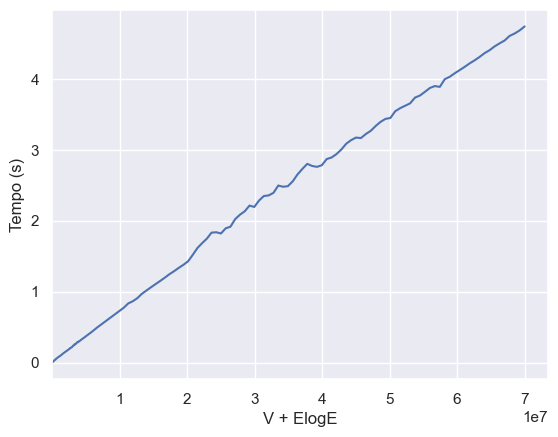
\includegraphics[width=4in]{report.png}
    \caption{Complexidade temporal do problema proposto}
  \end{figure}

  O gráfico apresentado tem o número de arestas no eixo dos $xx$ com uma escala $V + E \log E$ e o tempo em segundos no eixo dos $yy$.
  Os dados revelam uma tendência linear, comprovando que a complexidade temporal do problema é, num caso geral, $O(V + E\log E)$, tal como concluído na análise teórica.

  \printbibliography[title={Referência}]

\end{document}
